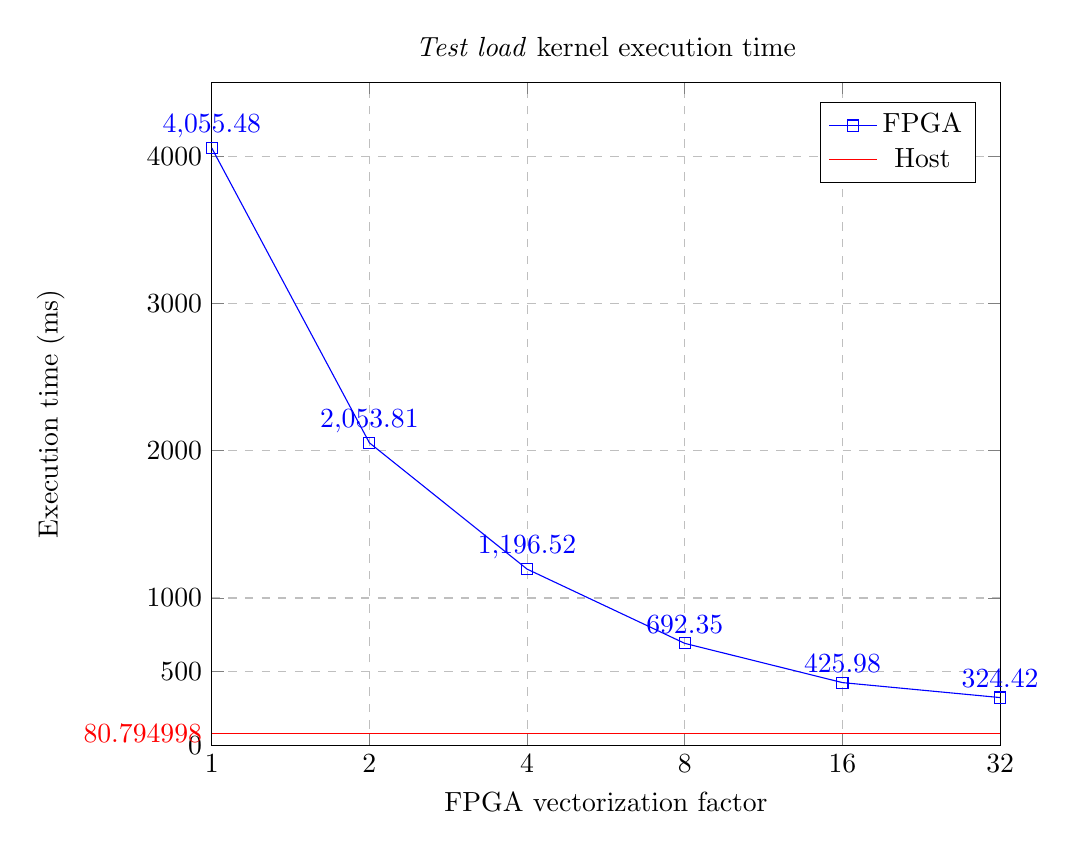
\begin{tikzpicture}
\begin{axis}[
    title={\textit{Test load} kernel execution time},
    xlabel={FPGA vectorization factor},
    ylabel={Execution time (ms)},
    xmin=1, xmax=6,
    ymin=0, ymax=4500,
    xticklabels={1,2,4,8,16,32},
    xtick={1,2,3,4,5,6},
    ytick={0,80.794998,500,1000,2000,3000,4000},
    yticklabels={0,\textcolor{red}{80.794998},500,1000,2000,3000,4000},
    legend pos=north east,
    xmajorgrids=true,
    ymajorgrids=true,
    grid style=dashed,
    height=10cm
]
\addplot[color=blue,mark=square, nodes near coords]
    coordinates {
        (1, 4055.47583) (2, 2053.811035) (3, 1196.515747) (4, 692.349365) (5, 425.979675) (6, 324.420349)
    };
    \addlegendentry{FPGA}

\addplot[color=red]
    coordinates {
        (1, 80.794998) (2, 80.794998) (3, 80.794998) (4, 80.794998) (5, 80.794998) (6, 80.794998)
    };
    \addlegendentry{Host}

\end{axis}
\end{tikzpicture}
